\section{Espansione}

\subsection{Aggiunta tripletta model-view-controller} \label{sec:aggiuntamvc}
Per inserire una tripletta mvc i passaggi verranno elencati prima nello specifico di ogni componente ed infine verrà esplicitato come collegare correttamente ogni componente. Per maggiori informazioni sulla struttura del codice fare riferimento a \S{}\ref{sec:cartelle-src}

\subsubsection{Aggiunta model}
Per aggiungere un nuovo model bisogna creare una nuova classe all'interno della cartella "model" che erediti dalla classe "\textit{QObject}". Se esso deve implementare il pattern singleton fare riferimento a \S{}\ref{sec:singleton-python}. La nuova componente del modello dovrà avere un segnale al suo interno per comunicare i cambiamenti del suo stato, il segnale è una variabile di classe istanziata con il seguente codice: \texttt{Sg\_model\_changed = Signal()} e ad ogni cambiamento di stato del modello deve essere segnalato emettendo un segnale così: \texttt{self.Sg\_model\_changed.emit()}.


\subsubsection{Aggiunta view}
Per aggiungere una nuova parte della view bisogna creare una nuova classe all'interno della cartella "view". Se si tratta di una view da rappresentare nella stessa finestra delle altre essa dovrà essere istanziata nel costruttore della classe \textit{"MainWidget"} e sempre nel costruttore essere aggiunto ai widget della classe. Il codice per l'aggiunta è il seguente: \newline{} \centerline{ \texttt{self.swidget.addWidget(new\_widget)}}.
Questa aggiunta viene mostrata con una sottolineatura nella seguente immagine:
\begin{figure}[H]
    \centering
    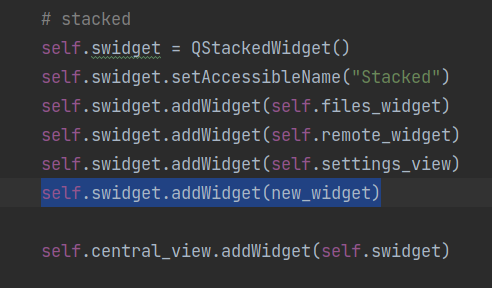
\includegraphics[scale = 0.75]{components/img/codice-nuova-view-su-main-view.png}
    \caption{Codice per inserimento nuova view nella main view}
    \label{fig:Codice per inserimento nuova view nella main view}
\end{figure}



\subsubsection{Aggiunta controller}

\subsubsection{Collegamento componenti}